\tikzstyle{block} = [rectangle, draw, minimum width=1.8cm, minimum height=1.5cm]
\tikzstyle{branch} = [circle, fill=black, minimum size=1mm, inner sep=0pt, node 
distance = 1cm]
\tikzstyle{connect} = [-latex, draw]
\tikzstyle{figure} = [inner sep=1, rectangle]

\begin{tikzpicture}
%% Nodes
\node[block] (spatial) {\shortstack{Spatial\\Bandwidth\\Limitation}};
\node[block,right=1.3cm of spatial] (synthesis) {\shortstack{2.5D\\Synthesis}};
\node[block,right=1.7cm of synthesis] (discrete) 
  {\shortstack{Spatial\\Discretisation}};
  
% inputs
\node[left=0.5cm of spatial, figure] (in1) {
\includegraphics[width=2cm]{fig1}};

% outputs
\node[below=0.5cm of spatial, figure] (out1)
  {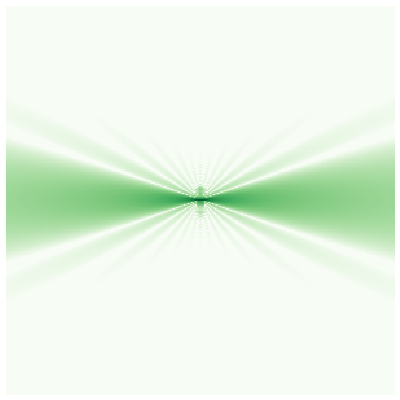
\includegraphics[width=2cm]{fig2}};
\node[below=0.5cm of synthesis, figure] (out2) 
  {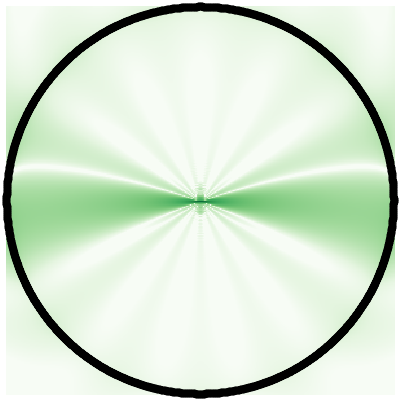
\includegraphics[width=2cm]{fig3}};
\node[below=0.5cm of discrete, figure] (out3)
  {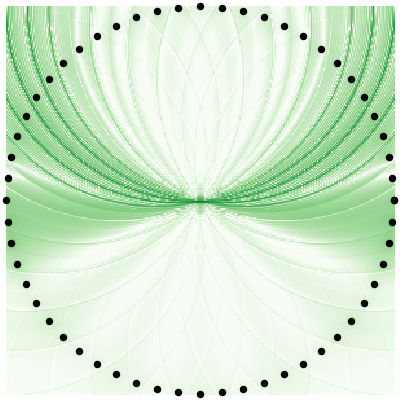
\includegraphics[width=2cm]{fig4}};
  
%% Connections
\draw[connect] (spatial) -- (synthesis)
  node[midway, above]{\footnotesize bandlimited} 
  node[midway, below]{\footnotesize sound field};
\draw[connect] (synthesis) -- (discrete)
  node[midway, above]{\footnotesize bandlimited} 
  node[midway, below]{\footnotesize driving function};

% inputs
\draw[connect] (in1) -- (spatial);

% outputs
\draw[connect] (spatial) -- (out1);
\draw[connect] (synthesis) -- (out2);
\draw[connect] (discrete) -- (out3);

\end{tikzpicture}